\section{Methodology}
The methodology for the Travel Agency website project follows a structured approach to ensure its success. First, a comprehensive review of existing travel agency systems will be conducted to identify gaps and limitations, which will inform the specific requirements of the system. Both functional and non-functional requirements will be defined, covering essential features such as user registration, package selection, payment integration, and the administrative ability to manage packages and local tour guides. A feasibility study will assess the technical, operational, and economic viability of the project, ensuring the availability of resources, user acceptance, and cost-effectiveness. The system's design will be high-level, focusing on architecture, key features, and algorithms for core processes. Additionally, flowcharts will be created to visualize system functionality. This methodology will ensure the website meets user needs while being technically feasible and economically viable.

\subsection{Requirement Identification}
\begin{figure}[H]  % Use 'H' to fix the image position
    \centering
    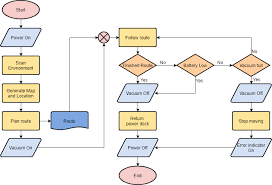
\includegraphics[width=0.5\linewidth]{./Images/flow.png}
    \caption{Requirement Identification Flowchart}
    \label{fig:Requirement Identification Flowchart}
\end{figure}



\subsubsection{Requirement Analysis}
\begin{itemize}
    \item \textbf{Technical Requirements}: The system must be built using \textbf{Next.js} for the frontend, \textbf{Laravel} for the backend, and \textbf{MySQL} for database management. It will require integration with a secure third-party payment gateway such as \textbf{Stripe} or \textbf{PayPal}.
    \item \textbf{Operational Requirements}: The system must be easy to use for both customers and administrators. Customers should be able to browse and book packages seamlessly, while administrators should have an intuitive interface for managing content and user data.
    \item \textbf{User Requirements}: The platform must support responsive design, allowing users to access the site from both desktop and mobile devices. It should also ensure data privacy and security for user accounts and payments.
\end{itemize}

\subsection{Functional Requirements}

The following table outlines the functional requirements for the Travel Agency website:

\begin{table}[h]
    \caption{Functional Requirements of the Travel Agency Website}
    \vspace{0.2in}
    \centering
    \begin{tabular}{|>{\raggedright\arraybackslash}p{5cm}|>{\raggedright\arraybackslash}p{9cm}|} % p{} for controlled column width, aligned text
        \hline
        \textbf{Feature} & \textbf{Use Case Scenario} \\
        \hline
        \textbf{User Registration} & Users must be able to create an account, log in, and reset their password. \\
        \hline
        \textbf{Package Browsing} & Users can view available tour packages, including package details, destinations, pricing, and itinerary. \\
        \hline
        \textbf{Package Selection} & Users can select a tour package, specify flight and hotel preferences, and proceed to the payment gateway. \\
        \hline
        \textbf{Payment Integration} & Users can complete their booking through a secure payment gateway (e.g., Stripe/PayPal). \\
        \hline
        \textbf{Admin CRUD Operations} & Admins can add, update, or delete tour packages and manage local tour guide information. \\
        \hline
        \textbf{User Dashboard} & Users can view their booking history, saved packages, and profile settings. \\
        \hline
    \end{tabular}
\end{table}

\newpage

\subsection{Non-Functional Requirements}
The following table lists the non-functional requirements for the system:
\begin{table}[h]
    \caption{Non-Functional Requirements of the Travel Agency Website}
    \vspace{0.2in}
    \centering
    \begin{tabular}{|>{\raggedright\arraybackslash}p{5cm}|>{\raggedright\arraybackslash}p{9cm}|}% Adjusted column width
        \hline
        \textbf{Requirement} & \textbf{Description} \\ 
        \hline
        \textbf{Performance} & The website should load in under 2 seconds and handle up to 500 simultaneous users without issues. \\
        \hline
        \textbf{Scalability} & The system should be able to scale horizontally to accommodate future growth in users and data. \\
        \hline
        \textbf{Security} & The system must ensure secure data transactions using encryption and secure payment APIs. \\
        \hline
        \textbf{Usability} & The platform should be intuitive, with a user-friendly interface for both customers and administrators. \\
        \hline
        \textbf{Reliability} & The system should have an uptime of 99.9\% and handle faults gracefully with automatic recovery. \\
        \hline
    \end{tabular}
\end{table}

\subsection{Feasibility Study}

\subsubsection{Technical Feasibility}
The technical feasibility of this project is supported by the availability of modern web development tools and technologies. \textbf{Next.js}, \textbf{Node.js}, and \textbf{MySQL} are all well-established and widely supported technologies that will be used to build the platform. The integration of secure payment gateways such as \textbf{Stripe} or \textbf{PayPal} will be achieved using their respective APIs, which are readily available and extensively documented.

\subsubsection{Operational Feasibility}
The operational feasibility of the project is high. The system will be designed with ease of use in mind for both customers and administrators. User interfaces will be designed to be intuitive, and the admin panel will provide an efficient way for administrators to manage packages and guide details. The system will also be compatible with existing user devices, providing a responsive design for both desktop and mobile platforms.

\subsubsection{Economic Feasibility}
A cost-benefit analysis has been performed to evaluate the economic feasibility of the project. The expected development costs are around \$23,000, with an estimated total benefit of \$60,000. The net benefit from the project is expected to be around \$37,000, making the project financially viable.

\begin{table}[ht]
    \caption{Cost-Benefit Analysis of the Proposed Travel Agency Website}
    \vspace{0.2in}
    \label{tab:cost_benefit_analysis}
    \centering
    \begin{tabular}{|l|r|r|}
        \hline
        \textbf{Item Description} & \textbf{Cost (\$)} & \textbf{Benefit (\$)} \\
        \hline
        \textbf{Development Costs} & 15,000 & - \\
        \hline
        \textbf{Hardware Costs} & 5,000 & - \\
        \hline
        \textbf{Training Costs} & 2,000 & - \\
        \hline
        \textbf{Maintenance Costs} & 1,000 & - \\
        \hline
        \textbf{Total Costs} & 23,000 & - \\
        \hline
        \textbf{Increased Efficiency} & - & 30,000 \\
        \hline
        \textbf{Improved User Satisfaction} & - & 10,000 \\
        \hline
        \textbf{Revenue Increase} & - & 20,000 \\
        \hline
        \textbf{Total Benefits} & - & 60,000 \\
        \hline
        \textbf{Net Benefit} & 23,000 & 37,000 \\
        \hline
    \end{tabular}
\end{table}

\subsubsection{Schedule}
The project will be completed within 10-12 weeks. The Gantt chart below outlines the project timeline, with key milestones and tasks:

\begin{table}[ht]
    \caption{Project Schedule for the Travel Agency Website}
    \vspace{0.2in}
    \label{tab:project_schedule}
    \centering
    \resizebox{\textwidth}{!}{
    \begin{tabular}{|l|l|l|}
        \hline
        \textbf{Milestone} & \textbf{Task} & \textbf{Timeframe} \\
        \hline
        \textbf{Sprint 1} & System design, database setup, and frontend development & Week 1-3 \\
        \hline
        \textbf{Sprint 2} & Backend development (user authentication, tour package management) & Week 4-6 \\
        \hline
        \textbf{Sprint 3} & Payment gateway integration and admin panel implementation & Week 7-9 \\
        \hline
        \textbf{Sprint 4} & Testing, debugging, and final deployment & Week 10-12 \\
        \hline
    \end{tabular}
    }
\end{table}


\subsection{High-Level Design of System}

\subsubsection{Methodology of the Proposed System}
The proposed system will follow an \textbf{Object-Oriented} design approach to ensure modularity, scalability, and reusability. The system will consist of multiple classes representing users, packages, bookings, and administrative functions. Each class will interact with the database through models that handle data retrieval and storage.

\subsubsection{Flow Charts/Working Mechanism of the Proposed System}
\begin{figure}[H]  % Use 'H' to fix the image position
    \centering
    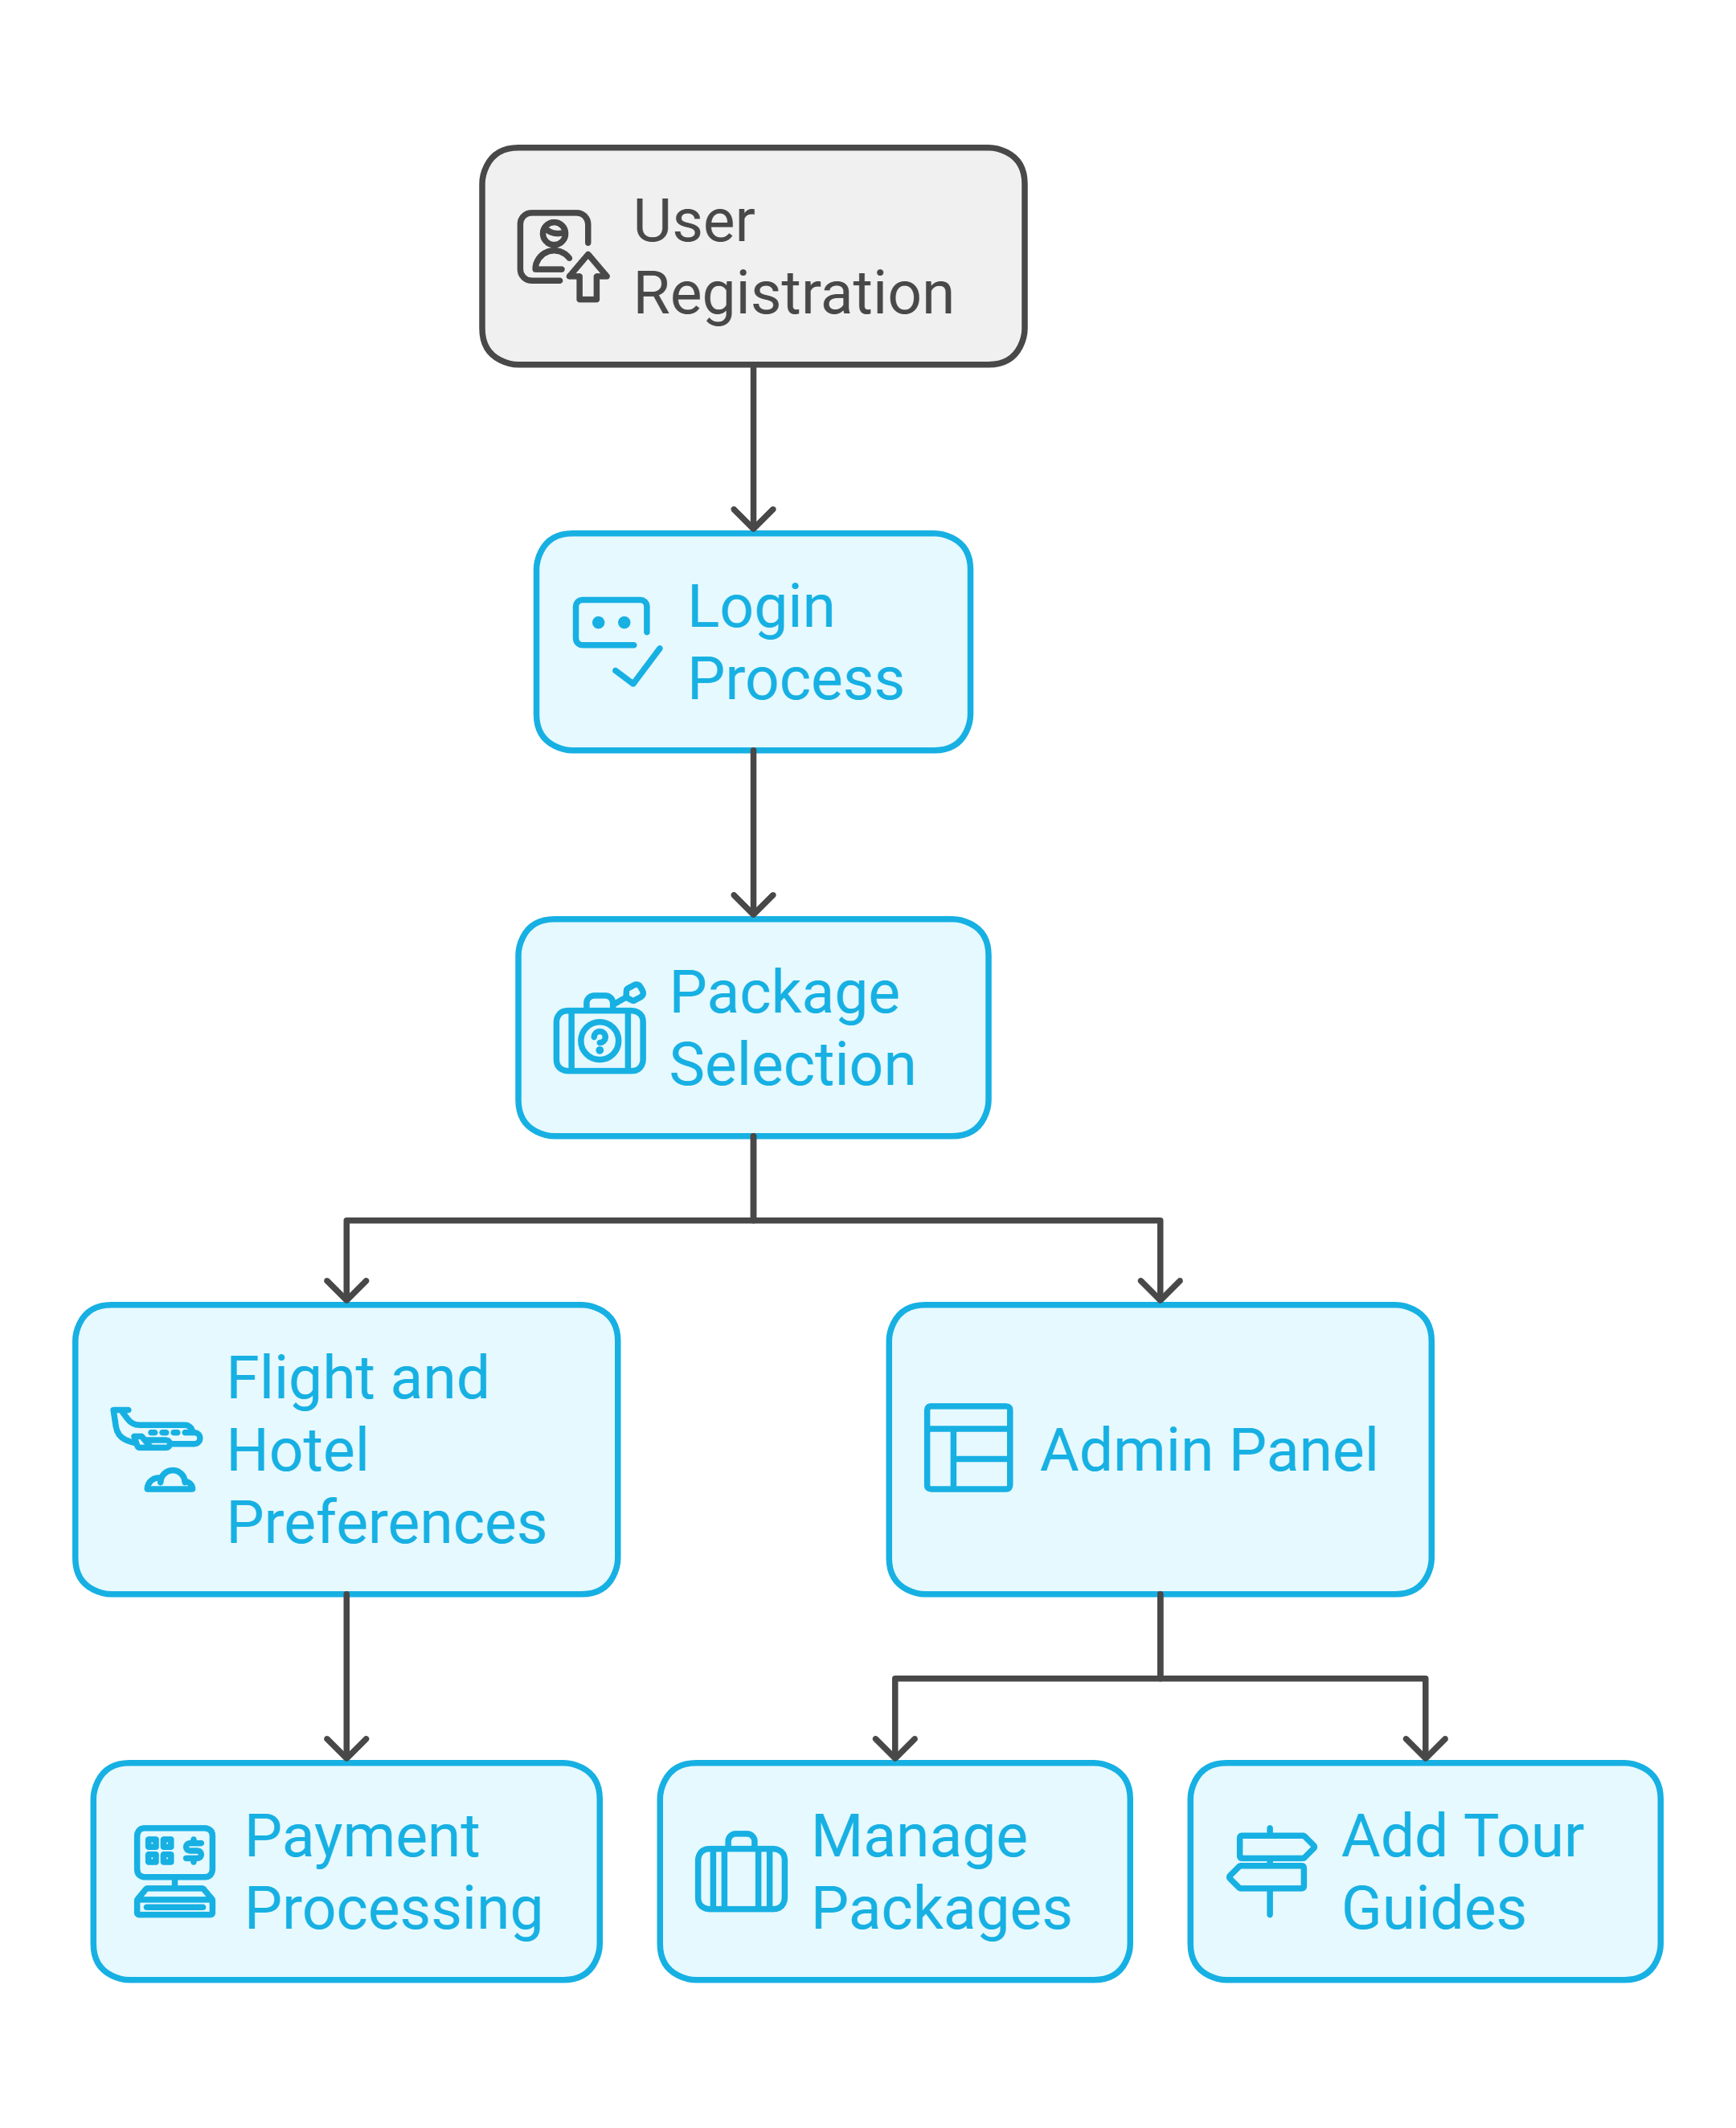
\includegraphics[width=0.5\linewidth]{./Images/flow2.png}
    \caption{Flowchart of the Proposed System}
    \label{fig:Requirement Identification Flowchart}
\end{figure}

\subsubsection{Description of Algorithms}
The primary algorithms for this system include:
\begin{itemize}
    \item \textbf{Authentication Algorithm}: Validates user credentials during login and handles session management.
    \item \textbf{Package Selection Algorithm}: Filters available packages based on user preferences and displays them in an optimized manner.
    \item \textbf{Payment Processing Algorithm}: Manages secure payment transactions, including interaction with the third-party payment gateway and confirmation of successful payment.
\end{itemize}
The system will leverage these algorithms to ensure a smooth and efficient user experience throughout the booking process.
